\chapter{Convoluciones y Atención---Perception as Transformation}

\begin{quote}
	\itshape
	``The eye sees only what the mind is prepared to comprehend.''
	
	\raggedleft--- Robertson Davies
\end{quote}

\begin{quote}
	\itshape
	``Vision is the art of seeing the invisible.''
	
	\raggedleft--- Jonathan Swift
\end{quote}

\section{Introduction: Vision as Active Construction}

Vision is not passive reception of light rays but \textit{active construction of meaning}. As Maurice Merleau-Ponty argued in \textit{Phenomenology of Perception} (1945), perception is embodied engagement with the world---we do not merely \textit{receive} visual data, we \textit{interrogate} it through attention, expectation, and memory.

Convolutional neural networks (CNNs) formalize this philosophical insight: perception is hierarchical feature detection, where local patterns (edges, textures) compose into global structures (objects, scenes). The notation of convolution captures this multi-scale synthesis.

\section{Convolution as Local-Global Synthesis}

\subsection{The Mathematical Definition}

\begin{seanbox}{3.1}
	\textbf{2D Convolution (Single Channel):}
	
	For input image $X \in \R^{H \times W}$ and kernel $K \in \R^{(2r+1) \times (2r+1)}$:
	
	\begin{equation}
		Y_{pq} = (K \ast X)_{pq} = \sum_{u=-r}^r \sum_{v=-r}^r K_{uv} \cdot X_{(p+u)(q+v)}
	\end{equation}
	
	\textbf{Multi-Channel Convolution:}
	
	For input $X \in \R^{H \times W \times C_{\text{in}}}$, kernel $K \in \R^{(2r+1) \times (2r+1) \times C_{\text{in}} \times C_{\text{out}}}$:
	
	\begin{equation}
		Y_{pqc_o} = \sum_{c=1}^{C_{\text{in}}} \sum_{u=-r}^r \sum_{v=-r}^r K_{uvc c_o} \cdot X_{(p+u)(q+v)c}
	\end{equation}
	
	\textbf{Notational Conventions:}
	\begin{itemize}
		\item Subscripts $p, q$: Spatial position (row, column) --- the \textit{where}
		\item Subscript $c$: Channel index (color, feature) --- the \textit{what}
		\item Subscripts $u, v$: Kernel offset (relative position within receptive field)
		\item $(2r+1) \times (2r+1)$: Kernel size (receptive field diameter)
	\end{itemize}
\end{seanbox}

\begin{philobox}
	\textbf{Philosophical Intuition: Locality and Universality}
	
	Convolution embodies a profound tension in epistemology:
	
	\begin{enumerate}
		\item \textbf{Locality}: Each output $Y_{pq}$ depends only on a \textit{local neighborhood} of input---the receptive field centered at $(p,q)$. This is spatial \textit{particularity}: features are grounded in specific locations.
		
		\item \textbf{Universality}: The \textit{same} kernel $K$ is applied everywhere---translation invariance. This is the Platonic \textit{universal}: one form (the kernel) manifests across many particulars (image locations).
	\end{enumerate}
	
	This mirrors Merleau-Ponty's \textit{body schema}: perception is neither purely local (atomistic sense data) nor purely global (abstract concepts) but a \textit{structured field} where local and global interpenetrate.
	
	The notation $K_{uvc c_o}$ makes this synthesis explicit:
	\begin{itemize}
		\item Indices $u, v$: Local spatial structure (receptive field geometry)
		\item Index $c$: Local feature channel (what is being detected)
		\item Index $c_o$: Global semantic category (output feature map)
	\end{itemize}
	
	Convolution is the mathematical formalization of \textit{structured attention}: each kernel is a question asked of the image, and convolution is the process of asking that question everywhere.
\end{philobox}

\subsection{Historical Depth: From Hubel-Wiesel to Deep Learning}

\subsubsection{Hubel \& Wiesel (1962): The Biological Inspiration}

David Hubel and Torsten Wiesel discovered that neurons in cat visual cortex have \textit{receptive fields}---they respond selectively to oriented edges in specific retinal locations. This revolutionized neuroscience by showing that vision is \textit{hierarchical}:

\begin{itemize}
	\item \textbf{Simple cells}: Detect oriented edges (vertical, horizontal, diagonal)
	\item \textbf{Complex cells}: Detect edges with position invariance
	\item \textbf{Hypercomplex cells}: Detect corners, end-stopping
\end{itemize}

\begin{remark}[The Philosophical Significance]
	Hubel and Wiesel showed that perception is \textit{constructive}, not passive. The brain doesn't receive a ``picture'' but actively extracts features through hierarchical filtering. This vindicated Kant's insight: intuition (Anschauung) imposes structure on sensation.
\end{remark}

\subsubsection{Fukushima's Neocognitron (1980): First Hierarchical CNN}

Inspired by Hubel-Wiesel, Kunihiko Fukushima designed the \textit{Neocognitron}---a hierarchical neural network with:
\begin{itemize}
	\item \textbf{S-layers}: Feature extraction (convolution-like)
	\item \textbf{C-layers}: Position invariance (pooling-like)
\end{itemize}

Though not trained with backpropagation, it demonstrated that visual recognition could emerge from hierarchical, locally-connected networks.

\subsubsection{LeCun's LeNet (1989): The Birth of Modern CNNs}

Yann LeCun combined Fukushima's architecture with backpropagation, creating LeNet---the first CNN trained end-to-end for digit recognition (MNIST). Key innovations:

\begin{enumerate}
	\item \textbf{Weight sharing}: Same kernel everywhere (convolution)
	\item \textbf{Backpropagation}: Gradient descent through the entire network
	\item \textbf{Pooling}: Subsampling for translation invariance
\end{enumerate}

LeNet's notation $y_{pq}^{(\ell)} = \sigma(\sum_c \sum_{uv} w_{uvc}^{(\ell)} \cdot x_{(p+u)(q+v)c}^{(\ell-1)})$ made explicit the compositional structure of vision.

\subsubsection{AlexNet (2012): The Deep Learning Revolution}

Alex Krizhevsky, Ilya Sutskever, and Geoffrey Hinton scaled CNNs to ImageNet (1.2 million images, 1000 categories), achieving 15.3\% top-5 error---far surpassing previous methods (26\%). Key innovations:

\begin{itemize}
	\item \textbf{ReLU activation}: $\sigma(z) = \max(0, z)$ instead of sigmoid
	\item \textbf{Dropout}: Regularization by randomly dropping units
	\item \textbf{GPU acceleration}: Parallel computation on NVIDIA GTX 580
	\item \textbf{Data augmentation}: Translations, flips, color jittering
\end{itemize}

AlexNet proved that deep CNNs could match human-level vision, inaugurating the current AI era.

\subsection{Convolution as Correlation and Cross-Correlation}

\begin{notation}[Convolution vs. Cross-Correlation]
	In signal processing, \textit{convolution} involves flipping the kernel:
	\begin{equation}
		(f \ast g)(t) = \int_{-\infty}^\infty f(\tau) g(t - \tau) d\tau
	\end{equation}
	
	In deep learning, what we call ``convolution'' is technically \textit{cross-correlation} (no flip):
	\begin{equation}
		Y_{pq} = \sum_{u,v} K_{uv} X_{(p+u)(q+v)}
	\end{equation}
	
	\textbf{Why the difference?} In CNNs, kernels are \textit{learned}, so flipping is unnecessary---the network learns the appropriate orientation. The term ``convolution'' is retained by convention.
\end{notation}

\begin{philosophical}
	This notational slippage reveals a deeper truth: \textit{mathematical operations acquire meaning through use}. In signal processing, convolution's kernel-flip encodes physical causality (time reversal in filtering). In neural networks, the operation signifies \textit{feature detection}---no flip needed because features are symmetric under learning.
	
	Wittgenstein's \textit{meaning as use}: the same notation ($\ast$) has different semantics in different language games.
\end{philosophical}

\subsection{Receptive Fields and Hierarchical Composition}

\begin{definition}[Receptive Field]
	The \textit{receptive field} of a neuron is the region of input space that affects its activation. For a convolution layer with kernel size $(2r+1) \times (2r+1)$, each output neuron's receptive field is $(2r+1) \times (2r+1)$.
	
	In deep networks, receptive fields \textit{grow} with depth:
	\begin{equation}
		\text{RF}_\ell = \text{RF}_{\ell-1} + 2r_\ell \cdot \prod_{k=1}^{\ell-1} s_k
	\end{equation}
	where $r_\ell$ is kernel radius at layer $\ell$, $s_k$ is stride at layer $k$.
\end{definition}

\begin{visualbox}
	\textbf{Hierarchical Receptive Fields:}
	
	\begin{center}
		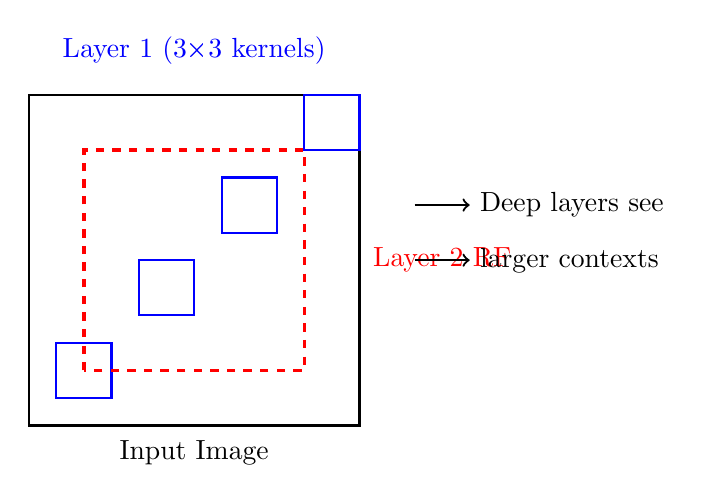
\begin{tikzpicture}[scale=0.7]
			% Layer 1: Input
			\draw[thick] (0,0) rectangle (6,6);
			\node at (3, -0.5) {Input Image};
			
			% Layer 2: First conv (small RFs)
			\foreach \x in {0.5, 2, 3.5, 5} {
				\draw[blue, thick] (\x, \x) rectangle (\x+1, \x+1);
			}
			\node[blue] at (3, 6.8) {Layer 1 (3×3 kernels)};
			
			% Layer 3: Second conv (larger RFs)
			\draw[red, very thick, dashed] (1, 1) rectangle (5, 5);
			\node[red] at (7.5, 3) {Layer 2 RF};
			
			% Arrows showing composition
			\draw[->, thick] (7, 4) -- (8, 4) node[right] {Deep layers see};
			\draw[->, thick] (7, 3) -- (8, 3) node[right] {larger contexts};
		\end{tikzpicture}
	\end{center}
	
	As depth increases, each neuron integrates information from increasingly large image regions---\textit{compositional abstraction}.
\end{visualbox}

\begin{philosophical}
	This hierarchy echoes Gestalt psychology's principle: ``The whole is other than the sum of its parts.'' Early layers detect edges (local parts), deep layers detect objects (global wholes). The notation $Y^{(\ell)}$ (output at layer $\ell$) captures this \textit{emergence}---higher levels are not reducible to lower levels but arise from their composition.
	
	In Hegelian dialectics: thesis (pixels) + antithesis (local edges) = synthesis (global objects).
\end{philosophical}

\section{Padding, Stride, and Dilation: Geometries of Attention}

\subsection{Padding: Preserving Spatial Structure}

\begin{seanbox}{3.2}
	\textbf{Padding Types:}
	
	\textbf{Valid (No Padding):}
	\begin{equation}
		\text{Output size} = \lfloor \frac{H - K + 1}{s} \rfloor \times \lfloor \frac{W - K + 1}{s} \rfloor
	\end{equation}
	
	\textbf{Same (Zero Padding):}
	Pad input with $p = \lfloor K/2 \rfloor$ zeros on each side to preserve size:
	\begin{equation}
		\text{Output size} = \lfloor \frac{H + 2p - K + 1}{s} \rfloor = H \times W \quad (\text{if } s=1)
	\end{equation}
	
	\textbf{Notation:} $X_{\text{padded}} = \text{pad}(X, p)$
\end{seanbox}

\begin{philosophical}
	Padding is a \textit{boundary condition}---a metaphysical choice about how to treat edges. Zero padding assumes ``nothing beyond the frame'' (existential finitude). Reflection padding (mirror edges) assumes symmetry. Circular padding (wrap around) assumes periodicity.
	
	This echoes Kant's \textit{antinomies of pure reason}: does space have boundaries (finite) or extend infinitely? Padding formalizes our answer.
\end{philosophical}

\subsection{Stride: Subsampling Attention}

\begin{seanbox}{3.3}
	\textbf{Strided Convolution:}
	
	Instead of shifting kernel by 1 pixel, shift by $s$ pixels (stride):
	\begin{equation}
		Y_{pq} = \sum_{u,v} K_{uv} X_{(sp+u)(sq+v)}
	\end{equation}
	
	\textbf{Effect:} Reduces spatial dimensions by factor of $s$:
	\begin{equation}
		H_{\text{out}} = \lfloor \frac{H_{\text{in}} - K}{s} \rfloor + 1
	\end{equation}
\end{seanbox}

\begin{philosophical}
	Stride is \textit{selective inattention}---we skip intermediate positions, focusing only on spaced-out locations. This is William James' \textit{stream of consciousness}: attention cannot grasp everything, so it samples strategically.
	
	In phenomenology, this is Husserl's \textit{horizon structure}: the attentional foreground (sampled locations) against a background (skipped locations).
\end{philosophical}

\subsection{Dilation: Expanding the Receptive Field}

\begin{seanbox}{3.4}
	\textbf{Dilated (Atrous) Convolution:}
	
	Insert gaps between kernel elements (dilation rate $d$):
	\begin{equation}
		Y_{pq} = \sum_{u=-r}^r \sum_{v=-r}^r K_{uv} X_{(p+du)(q+dv)}
	\end{equation}
	
	\textbf{Effect:} Expands receptive field without increasing parameters:
	\begin{equation}
		\text{Effective kernel size} = K + (K-1)(d-1)
	\end{equation}
	
	Example: $3 \times 3$ kernel with $d=2$ has $5 \times 5$ receptive field.
\end{seanbox}

\begin{visualbox}
	\textbf{Dilation Visualization:}
	
	\begin{center}
		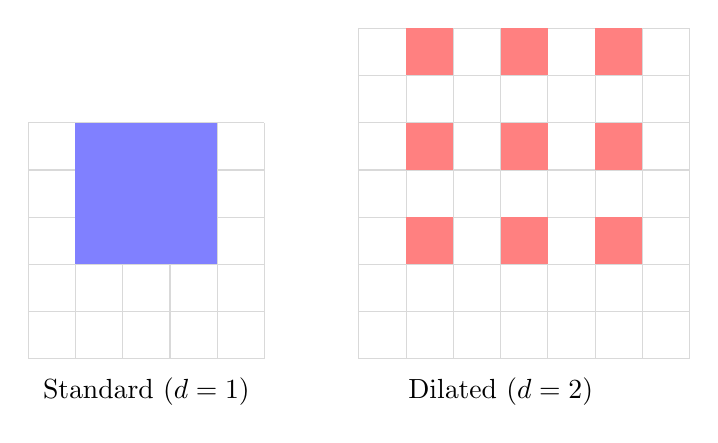
\begin{tikzpicture}[scale=0.6]
			% Standard convolution
			\draw[step=1cm, gray!30] (0,0) grid (5,5);
			\foreach \x/\y in {1/2, 2/2, 3/2, 1/3, 2/3, 3/3, 1/4, 2/4, 3/4} {
				\fill[blue!50] (\x,\y) rectangle (\x+1,\y+1);
			}
			\node at (2.5, -0.7) {Standard ($d=1$)};
			
			% Dilated convolution
			\begin{scope}[xshift=7cm]
				\draw[step=1cm, gray!30] (0,0) grid (7,7);
				\foreach \x/\y in {1/2, 3/2, 5/2, 1/4, 3/4, 5/4, 1/6, 3/6, 5/6} {
					\fill[red!50] (\x,\y) rectangle (\x+1,\y+1);
				}
				\node at (3, -0.7) {Dilated ($d=2$)};
			\end{scope}
		\end{tikzpicture}
	\end{center}
	
	Dilation spreads receptive field while maintaining parameter count---\textit{efficiency through sparsity}.
\end{visualbox}

\begin{philosophical}
	Dilation is \textit{scale-invariant attention}---detecting patterns at multiple scales without explicit downsampling. This resonates with fractal geometry (Mandelbrot): self-similarity across scales.
	
	In cognitive science, this is \textit{coarse coding}: sparse sampling that still captures global structure.
\end{philosophical}

\section{Batch Normalization: Stabilizing the Perceptual Flow}

\subsection{The Covariate Shift Problem}

\begin{definition}[Internal Covariate Shift]
	As lower layers of a network learn, their output distributions change, forcing upper layers to continuously adapt. This \textit{internal covariate shift} slows training and destabilizes gradients.
\end{definition}

\begin{philosophical}
	This is the \textit{problem of flux} (Heraclitus): ``You cannot step into the same river twice.'' Each layer experiences a non-stationary input distribution---the ``ground shifts beneath its feet.'' Learning becomes a moving target.
	
	Batch Normalization addresses this by imposing \textit{statistical regularity}---a Kantian \textit{synthetic a priori} structure.
\end{philosophical}

\subsection{The Batch Normalization Transformation}

\begin{seanbox}{3.5}
	\textbf{Batch Normalization (BN):}
	
	Given mini-batch $\{x^{(i)}\}_{i=1}^m$ and feature index $j$:
	
	\textbf{Step 1: Compute batch statistics}
	\begin{align}
		\mu_j^{\mathcal{B}} &= \frac{1}{m} \sum_{i=1}^m x_j^{(i)} \quad \text{(batch mean)} \\
		(\sigma_j^{\mathcal{B}})^2 &= \frac{1}{m} \sum_{i=1}^m (x_j^{(i)} - \mu_j^{\mathcal{B}})^2 \quad \text{(batch variance)}
	\end{align}
	
	\textbf{Step 2: Normalize}
	\begin{equation}
		\hat{x}_j^{(i)} = \frac{x_j^{(i)} - \mu_j^{\mathcal{B}}}{\sqrt{(\sigma_j^{\mathcal{B}})^2 + \epsilon}}
	\end{equation}
	where $\epsilon$ (e.g., $10^{-5}$) prevents division by zero.
	
	\textbf{Step 3: Scale and shift (learnable affine transformation)}
	\begin{equation}
		y_j^{(i)} = \gamma_j \hat{x}_j^{(i)} + \beta_j
	\end{equation}
	where $\gamma_j, \beta_j$ are learnable parameters.
	
	\textbf{Notational Significance:}
	\begin{itemize}
		\item Superscript $\mathcal{B}$: Statistics computed over \textit{batch} (not population)
		\item Hat $\hat{x}$: Normalized activations (zero mean, unit variance)
		\item Tilde $\tilde{x}$: Often used for final transformed activations
	\end{itemize}
\end{seanbox}

\begin{philobox}
	\textbf{The Philosophy of Normalization}
	
	Batch Normalization is \textbf{perceptual homeostasis}---maintaining stable internal representations despite external flux. Three philosophical levels:
	
	\begin{enumerate}
		\item \textbf{Epistemological}: Normalization is \textit{standardization of measurement}. Just as scientists use standard units (meters, seconds), BN enforces standard activations (zero mean, unit variance). This is the Enlightenment ideal: universal, objective measures.
		
		\item \textbf{Ontological}: The learnable parameters $\gamma, \beta$ allow the network to \textit{undo} the normalization if beneficial. This is Hegelian \textit{Aufhebung} (sublation): standardization is both imposed and transcended.
		
		\item \textbf{Phenomenological}: BN stabilizes the \textit{attentional field}. In Husserl's terms, it establishes an \textit{invariant structure} (zero mean, unit variance) within which \textit{variations} ($\gamma, \beta$) can be meaningfully perceived.
	\end{enumerate}
	
	The notation $\mu^{\mathcal{B}}$ captures the \textit{contingency} of batch statistics---they are sample-based, not ground truth. This is statistical epistemology: knowledge is probabilistic, not absolute.
\end{philobox}

\subsection{Why Batch Normalization Works}

\begin{theorem}[Ioffe \& Szegedy, 2015]
	Batch Normalization enables:
	\begin{enumerate}
		\item \textbf{Higher learning rates}: Gradients are better scaled
		\item \textbf{Reduced sensitivity to initialization}: Normalization stabilizes early training
		\item \textbf{Regularization effect}: Noise in batch statistics acts like dropout
		\item \textbf{Gradient flow}: Prevents vanishing/exploding gradients
	\end{enumerate}
\end{theorem}

\begin{remark}[Recent Understanding]
	Recent work (Santurkar et al., 2018) suggests BN's primary benefit is \textit{smoothing the loss landscape}---making optimization easier by reducing sensitivity to parameter changes. The ``covariate shift'' explanation may be secondary.
\end{remark}

\subsection{Inference Mode: Population Statistics}

\begin{notation}[Train vs. Test]
	During \textbf{training}, use batch statistics $\mu^{\mathcal{B}}, (\sigma^{\mathcal{B}})^2$.
	
	During \textbf{inference}, use population statistics (running averages):
	\begin{align}
		\mu_{\text{pop}} &= \E_{\mathcal{B}}[\mu^{\mathcal{B}}] \approx \text{running\_mean} \\
		\sigma^2_{\text{pop}} &= \E_{\mathcal{B}}[(\sigma^{\mathcal{B}})^2] \approx \text{running\_var}
	\end{align}
	
	This ensures deterministic behavior at test time (no randomness from batch sampling).
\end{notation}

\begin{philosophical}
	The train/test distinction mirrors \textit{induction vs. deduction}:
	\begin{itemize}
		\item \textbf{Training}: Inductive---learn from particular batches
		\item \textbf{Testing}: Deductive---apply general population statistics
	\end{itemize}
	
	This is Hume's problem of induction: how do we justify generalizing from seen (training batches) to unseen (test data)? BN's answer: accumulate statistics over many batches (law of large numbers).
\end{philosophical}

\section{Self-Attention: Content-Based Associative Memory}

\subsection{The Attention Mechanism}

\begin{seanbox}{3.6}
	\textbf{Scaled Dot-Product Attention:}
	
	Given input sequence $X \in \R^{n \times d}$ (n tokens, d-dimensional embeddings):
	
	\textbf{Step 1: Compute Query, Key, Value}
	\begin{align}
		Q &= X W^Q \in \R^{n \times d_k} \quad \text{(queries: what to look for)} \\
		K &= X W^K \in \R^{n \times d_k} \quad \text{(keys: what is being looked at)} \\
		V &= X W^V \in \R^{n \times d_v} \quad \text{(values: information to retrieve)}
	\end{align}
	
	\textbf{Step 2: Compute attention scores}
	\begin{equation}
		S = \frac{QK^\top}{\sqrt{d_k}} \in \R^{n \times n}
	\end{equation}
	
	\textbf{Step 3: Apply softmax (convert to probabilities)}
	\begin{equation}
		A = \softmax(S) = \left[\frac{\exp(S_{ij})}{\sum_{j'} \exp(S_{ij'})}\right] \in \R^{n \times n}
	\end{equation}
	
	\textbf{Step 4: Aggregate values}
	\begin{equation}
		\text{Output} = AV \in \R^{n \times d_v}
	\end{equation}
	
	\textbf{Complete Formula:}
	\begin{equation}
		\text{Attention}(Q, K, V) = \softmax\left(\frac{QK^\top}{\sqrt{d_k}}\right) V
	\end{equation}
\end{seanbox}

\begin{philobox}
	\textbf{Attention as Intentionality}
	
	Attention is \textbf{consciousness directed toward an object} (Husserl's \textit{Intentionalität}). The notation captures this:
	
	\begin{itemize}
		\item \textbf{Query $Q_i$}: The \textit{noesis} (act of intending)---what is sought
		\item \textbf{Key $K_j$}: The \textit{noema} (intended object)---what is available
		\item \textbf{Value $V_j$}: The \textit{hyle} (sensory content)---what is retrieved
		\item \textbf{Attention weight $A_{ij}$}: The \textit{degree of givenness}---how relevant $j$ is to $i$
	\end{itemize}
	
	The dot product $Q_i \cdot K_j$ measures \textit{resonance}---how much query $i$ ``recognizes'' key $j$. This is Plato's \textit{anamnesis} (recollection): the soul recognizes what it already knew.
	
	Softmax ensures $\sum_j A_{ij} = 1$---attention is \textit{selective}, not exhaustive. We cannot attend to everything (William James: ``My experience is what I agree to attend to'').
	
	The scaling $1/\sqrt{d_k}$ prevents saturation when $d_k$ is large---a technical detail with philosophical import: \textit{high-dimensional spaces need normalization to remain interpretable}.
\end{philobox}

\subsection{Why Attention Works: The Geometry of Similarity}

\begin{proposition}[Dot Product as Cosine Similarity]
	If $Q_i, K_j$ are normalized ($\|Q_i\| = \|K_j\| = 1$), then:
	\begin{equation}
		Q_i \cdot K_j = \cos(\theta_{ij})
	\end{equation}
	where $\theta_{ij}$ is the angle between vectors.
	
	\textbf{Interpretation:} Attention weights measure \textit{angular alignment}---vectors pointing in similar directions have high attention.
\end{proposition}

\begin{visualbox}
	\textbf{Attention as Angular Alignment:}
	
	\begin{center}
		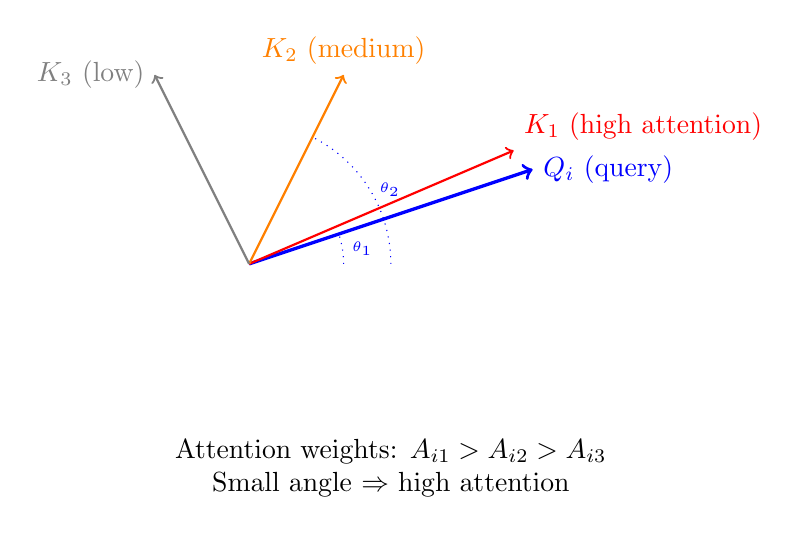
\begin{tikzpicture}[scale=1.2]
			% Origin
			\coordinate (O) at (0,0);
			
			% Query vector
			\draw[->, very thick, blue] (O) -- (3, 1) node[right] {$Q_i$ (query)};
			
			% Key vectors
			\draw[->, thick, red] (O) -- (2.8, 1.2) node[above right] {$K_1$ (high attention)};
			\draw[->, thick, orange] (O) -- (1, 2) node[above] {$K_2$ (medium)};
			\draw[->, thick, gray] (O) -- (-1, 2) node[left] {$K_3$ (low)};
			
			% Angles
			\draw[dotted, blue] (1, 0) arc (0:18:1) node[midway, right] {\tiny $\theta_1$};
			\draw[dotted, blue] (1.5, 0) arc (0:63:1.5) node[midway, right] {\tiny $\theta_2$};
			
			\node[below=1.5cm, align=center] at (1.5, -0.5) {
				Attention weights: $A_{i1} > A_{i2} > A_{i3}$ \\
				Small angle $\Rightarrow$ high attention
			};
		\end{tikzpicture}
	\end{center}
\end{visualbox}

\subsection{Multi-Head Attention: Parallel Perspectives}

\begin{seanbox}{3.7}
	\textbf{Multi-Head Attention:}
	
	Compute $h$ attention heads in parallel, each with different projections:
	
	\begin{equation}
		\text{head}_i = \text{Attention}(XW_i^Q, XW_i^K, XW_i^V)
	\end{equation}
	
	Concatenate and project:
	\begin{equation}
		\text{MultiHead}(X) = \text{Concat}(\text{head}_1, \ldots, \text{head}_h) W^O
	\end{equation}
	
	Each head learns different aspects (syntax, semantics, coreference, etc.).
\end{seanbox}

\begin{philosophical}
	Multi-head attention is \textbf{perspectivism} (Nietzsche): there is no single correct way to attend---multiple simultaneous perspectives enrich understanding.
	
	Each head is a \textit{Fragestellung} (mode of questioning). In Heidegger's hermeneutics, interpretation requires multiple readings---the meaning of text emerges from their synthesis.
\end{philosophical}

\section{3D Geometry: Rotations and Projections}

\subsection{The Special Orthogonal Group SO(3)}

\begin{seanbox}{3.8}
	\textbf{Rotation Group:}
	
	\begin{equation}
		SO(3) = \{ R \in \R^{3 \times 3} : R^\top R = I, \det(R) = 1 \}
	\end{equation}
	
	\textbf{Properties:}
	\begin{itemize}
		\item $R^\top R = I$: Orthogonality (preserves lengths and angles)
		\item $\det(R) = 1$: Orientation-preserving (right-handed)
		\item Closed under composition: $R_1, R_2 \in SO(3) \Rightarrow R_1 R_2 \in SO(3)$
	\end{itemize}
	
	\textbf{Euler Angle Parameterization:}
	\begin{align}
		R_x(\alpha) &= \begin{bmatrix} 1 & 0 & 0 \\ 0 & \cos\alpha & -\sin\alpha \\ 0 & \sin\alpha & \cos\alpha \end{bmatrix} \\
		R_y(\beta) &= \begin{bmatrix} \cos\beta & 0 & \sin\beta \\ 0 & 1 & 0 \\ -\sin\beta & 0 & \cos\beta \end{bmatrix} \\
		R_z(\gamma) &= \begin{bmatrix} \cos\gamma & -\sin\gamma & 0 \\ \sin\gamma & \cos\gamma & 0 \\ 0 & 0 & 1 \end{bmatrix}
	\end{align}
\end{seanbox}

\begin{philobox}
	\textbf{Rotations as Invariance}
	
	$SO(3)$ formalizes \textit{rotational symmetry}---the insight that physical laws don't depend on orientation. This is Noether's theorem: continuous symmetries correspond to conserved quantities (angular momentum).
	
	Philosophically, rotations capture \textit{the relativity of perspective}: different observers (rotated frames) see different coordinates for the same object, yet \textit{intrinsic properties} (lengths, angles) remain invariant.
	
	The notation $R \in SO(3)$ emphasizes \textit{membership in a structured space}---rotations form a Lie group (smooth manifold + group structure). This is the mathematics of continuous transformation.
\end{philobox}

\subsection{Pinhole Camera Model}

\begin{seanbox}{3.9}
	\textbf{Camera Projection Equation:}
	
	\begin{equation}
		\lambda \tilde{\vect{x}} = K [R \mid \vect{t}] \tilde{\vect{X}}
	\end{equation}
	
	Where:
	\begin{itemize}
		\item $\tilde{\vect{X}} = [X, Y, Z, 1]^\top$: 3D world point (homogeneous coordinates)
		\item $[R \mid \vect{t}] \in \R^{3 \times 4}$: Extrinsic matrix (world $\to$ camera frame)
		\item $K \in \R^{3 \times 3}$: Intrinsic matrix (camera parameters)
		\item $\tilde{\vect{x}} = [u, v, 1]^\top$: 2D image point (homogeneous)
		\item $\lambda$: Depth (scale factor)
	\end{itemize}
	
	\textbf{Intrinsic Matrix:}
	\begin{equation}
		K = \begin{bmatrix}
			f_x & 0 & c_x \\
			0 & f_y & c_y \\
			0 & 0 & 1
		\end{bmatrix}
	\end{equation}
	where $f_x, f_y$ are focal lengths (in pixels), $(c_x, c_y)$ is the principal point.
	
	\textbf{Extrinsic Matrix:}
	\begin{equation}
		[R \mid \vect{t}] = \begin{bmatrix}
			r_{11} & r_{12} & r_{13} & t_x \\
			r_{21} & r_{22} & r_{23} & t_y \\
			r_{31} & r_{32} & r_{33} & t_z
		\end{bmatrix}
	\end{equation}
\end{seanbox}

\begin{philobox}
	\textbf{Projection as Dimensional Collapse}
	
	The pinhole camera equation is \textbf{Plato's Cave}---3D reality projects onto a 2D image plane, losing depth information. The notation captures three philosophical operations:
	
	\begin{enumerate}
		\item \textbf{Extrinsic transformation $[R \mid \vect{t}]$}: Perspective shift---moving from world coordinates to camera coordinates. This is Kant's \textit{Copernican revolution}: objects conform to our mode of cognition (frame of reference).
		
		\item \textbf{Perspective projection} (implicit in $\lambda$): The division by depth $Z$ that collapses 3D to 2D. This is the \textit{reduction} Husserl criticized---lived experience (3D embodiment) reduced to visual appearance (2D retina).
		
		\item \textbf{Intrinsic transformation $K$}: Camera-specific distortion---focal length determines field of view. This is the \textit{apparatus} (Heidegger's \textit{Gestell})---technology mediates perception.
	\end{enumerate}
	
	The homogeneous coordinate notation $\tilde{\vect{x}}$ (with tilde) emphasizes \textit{projective equivalence}: points $(x, y, 1)$ and $(2x, 2y, 2)$ represent the \textit{same} 2D location. This is class equivalence---many representations, one essence.
\end{philobox}

\subsection{From 3D to 2D: The Projection Derivation}

\begin{derivation}[Perspective Projection]
	Start with 3D point $\vect{X} = [X, Y, Z]^\top$ in world coordinates.
	
	\textbf{Step 1: Transform to camera coordinates}
	\begin{equation}
		\vect{X}_c = R(\vect{X} - \vect{C}) = R\vect{X} + \vect{t}
	\end{equation}
	where $\vect{C}$ is camera center, $\vect{t} = -R\vect{C}$.
	
	\textbf{Step 2: Perspective division}
	Project onto image plane at $Z_c = f$ (focal length):
	\begin{equation}
		x = f \frac{X_c}{Z_c}, \quad y = f \frac{Y_c}{Z_c}
	\end{equation}
	
	\textbf{Step 3: Apply intrinsic parameters}
	\begin{equation}
		u = f_x x + c_x, \quad v = f_y y + c_y
	\end{equation}
	
	Combining in matrix form:
	\begin{equation}
		\begin{bmatrix} u \\ v \\ 1 \end{bmatrix} \sim K[R \mid \vect{t}] \begin{bmatrix} X \\ Y \\ Z \\ 1 \end{bmatrix}
	\end{equation}
	where $\sim$ denotes equality up to scale.
\end{derivation}

\begin{visualbox}
	\textbf{Pinhole Camera Geometry:}
	
	\begin{center}
		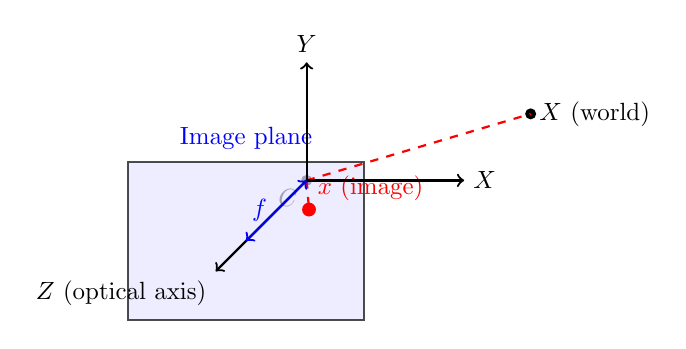
\begin{tikzpicture}[scale=1.0, every node/.style={scale=0.9}]
			% 3D coordinate system
			\coordinate (C) at (0,0,0);
			\coordinate (X) at (4,2,3);
			
			% Camera center
			\fill (C) circle (2pt) node[below left] {$C$};
			
			% Image plane
			\draw[thick, fill=blue!10, opacity=0.7] 
			(-1.5,-1,2) -- (1.5,-1,2) -- (1.5,1,2) -- (-1.5,1,2) -- cycle;
			\node[blue] at (0, 1.3, 2) {Image plane};
			
			% 3D point
			\fill (X) circle (2pt) node[right] {$\vect{X}$ (world)};
			
			% Projection ray
			\draw[dashed, thick, red] (C) -- (X);
			\draw[dashed, thick, red] (C) -- (0.8, 0.4, 2);
			
			% Projected point
			\fill[red] (0.8, 0.4, 2) circle (2.5pt) node[above right] {$\vect{x}$ (image)};
			
			% Axes
			\draw[->, thick] (C) -- (2,0,0) node[right] {$X$};
			\draw[->, thick] (C) -- (0,1.5,0) node[above] {$Y$};
			\draw[->, thick] (C) -- (0,0,3) node[below left] {$Z$ (optical axis)};
			
			% Focal length
			\draw[<->, thick, blue] (C) -- (0,0,2) node[midway, left] {$f$};
		\end{tikzpicture}
	\end{center}
	
	3D point projects onto image plane along ray from camera center.
\end{visualbox}

\section{Epipolar Geometry: The Mathematics of Stereo Vision}

\begin{seanbox}{3.10}
	\textbf{Fundamental Matrix:}
	
	Given two cameras viewing the same scene, the \textit{fundamental matrix} $F$ relates corresponding points:
	\begin{equation}
		\vect{x}_2^\top F \vect{x}_1 = 0
	\end{equation}
	
	\textbf{Geometric Meaning:} Point $\vect{x}_1$ in image 1 must lie on the \textit{epipolar line} in image 2, defined by $F\vect{x}_1$.
	
	\textbf{Essential Matrix:}
	If cameras are calibrated (intrinsics known):
	\begin{equation}
		E = K_2^\top F K_1, \quad E = [t]_\times R
	\end{equation}
	where $[t]_\times$ is the skew-symmetric matrix encoding translation.
\end{seanbox}

\begin{philosophical}
	Epipolar geometry formalizes \textit{perspectival consistency}: different viewpoints constrain each other. This is intersubjectivity (Husserl)---multiple subjects viewing the same object must have correlated experiences.
	
	The constraint $\vect{x}_2^\top F \vect{x}_1 = 0$ is a \textit{synthetic a priori} truth of stereo vision---it follows necessarily from projective geometry, independent of scene content.
\end{philosophical}

\section{Code Bridges: Manifesting Geometric Intuitions}

\subsection{Convolution in PyTorch}

\begin{codebox}
	\textbf{2D Convolution:}
	
	\begin{lstlisting}
		import torch
		import torch.nn.functional as F
		
		# Input: (batch, channels, height, width)
		X = torch.randn(1, 3, 32, 32)  # 1 RGB image, 32x32
		
		# Kernel: (out_channels, in_channels, kernel_h, kernel_w)
		K = torch.randn(64, 3, 3, 3)  # 64 filters, 3x3 each
		
		# Convolution with padding and stride
		Y = F.conv2d(X, K, padding=1, stride=1)
		
		print(f"Input shape: {X.shape}")    # [1, 3, 32, 32]
		print(f"Kernel shape: {K.shape}")   # [64, 3, 3, 3]
		print(f"Output shape: {Y.shape}")   # [1, 64, 32, 32]
		
		# With stride=2 (downsampling)
		Y_strided = F.conv2d(X, K, padding=1, stride=2)
		print(f"Strided output: {Y_strided.shape}")  # [1, 64, 16, 16]
	\end{lstlisting}
	
	\textbf{Philosophical Meditation:} Run this code and observe how padding and stride change output dimensions. Convolution is \textit{structure-preserving transformation}---spatial relationships maintained through hierarchical processing.
\end{codebox}

\subsection{Batch Normalization in Practice}

\begin{codebox}
	\begin{lstlisting}
		import torch
		import torch.nn as nn
		
		# Create BatchNorm layer (for 64 feature maps)
		bn = nn.BatchNorm2d(64)
		
		# Random activations (batch=32, channels=64, 16x16 spatial)
		x = torch.randn(32, 64, 16, 16)
		
		# Apply BatchNorm
		y = bn(x)
		
		# Verify normalization (per channel)
		for c in range(3):  # Check first 3 channels
		channel_mean = y[:, c, :, :].mean().item()
		channel_var = y[:, c, :, :].var(unbiased=False).item()
		print(f"Channel {c}: mean={channel_mean:.6f}, var={channel_var:.6f}")
		# Should be close to 0 and 1 (before gamma/beta)
		
		# Check learned parameters
		print(f"\nGamma (scale): {bn.weight[:5]}")  # First 5
		print(f"Beta (shift): {bn.bias[:5]}")
	\end{lstlisting}
	
	\textbf{Experiment:} Verify that each channel has approximately zero mean and unit variance after normalization.
\end{codebox}

\subsection{Self-Attention from Scratch}

\begin{codebox}
	\begin{lstlisting}
		import torch
		import torch.nn.functional as F
		
		def self_attention(X, d_k, d_v):
		"""
		X: (batch, seq_len, d_model) input sequence
		d_k: key/query dimension
		d_v: value dimension
		"""
		batch_size, seq_len, d_model = X.shape
		
		# Weight matrices (in practice, these are learned)
		W_Q = torch.randn(d_model, d_k)
		W_K = torch.randn(d_model, d_k)
		W_V = torch.randn(d_model, d_v)
		
		# Compute Q, K, V
		Q = X @ W_Q  # (batch, seq_len, d_k)
		K = X @ W_K  # (batch, seq_len, d_k)
		V = X @ W_V  # (batch, seq_len, d_v)
		
		# Scaled dot-product attention scores
		scores = Q @ K.transpose(-2, -1) / (d_k ** 0.5)  # (batch, seq_len, seq_len)
		
		# Apply softmax to get attention weights
		attn_weights = F.softmax(scores, dim=-1)  # (batch, seq_len, seq_len)
		
		# Weighted sum of values
		output = attn_weights @ V  # (batch, seq_len, d_v)
		
		return output, attn_weights
		
		# Example: sequence of 10 tokens, 64-dim embeddings
		X = torch.randn(2, 10, 64)  # batch=2
		output, attn = self_attention(X, d_k=64, d_v=64)
		
		print(f"Output shape: {output.shape}")  # [2, 10, 64]
		print(f"Attention shape: {attn.shape}")  # [2, 10, 10]
		print(f"\nAttention weights for first token:\n{attn[0, 0, :]}")
		print(f"Sum to 1: {attn[0, 0, :].sum()}")  # Should be 1.0
	\end{lstlisting}
	
	\textbf{Insight:} Each row of attention matrix shows how one token attends to all others---\textit{context-dependent weighting}.
\end{codebox}

\subsection{3D to 2D Projection}

\begin{codebox}
	\begin{lstlisting}
		import numpy as np
		
		def rotation_matrix_z(theta):
		"""Rotation around Z-axis"""
		c, s = np.cos(theta), np.sin(theta)
		return np.array([[c, -s, 0], [s, c, 0], [0, 0, 1]])
		
		def project_pinhole(X_world, R, t, K):
		"""
		Project 3D point to 2D image
		
		X_world: (3,) 3D point in world coordinates
		R: (3, 3) rotation matrix
		t: (3,) translation vector
		K: (3, 3) intrinsic matrix
		"""
		# Transform to camera coordinates
		X_cam = R @ X_world + t
		
		# Check if point is in front of camera
		if X_cam[2] <= 0:
		return None  # Behind camera
		
		# Perspective division
		x_normalized = X_cam[:2] / X_cam[2]
		
		# Apply intrinsics
		x_img = K[:2, :2] @ x_normalized + K[:2, 2]
		
		return x_img
		
		# Example: Project a 3D point
		X_world = np.array([1.0, 2.0, 5.0])  # 5 meters away
		
		# Camera rotation (30 degrees around Z)
		R = rotation_matrix_z(np.pi / 6)
		
		# Camera translation (no translation for simplicity)
		t = np.array([0.0, 0.0, 0.0])
		
		# Intrinsic matrix (focal length 800 pixels, center at 320x240)
		K = np.array([
		[800, 0, 320],
		[0, 800, 240],
		[0, 0, 1]
		])
		
		# Project
		x_img = project_pinhole(X_world, R, t, K)
		print(f"3D point {X_world} projects to pixel {x_img}")
		
		# Try projecting multiple points
		points_3d = np.array([
		[1, 0, 5],
		[0, 1, 5],
		[-1, 0, 5],
		[0, -1, 5]
		])
		
		print("\nProjecting multiple points:")
		for pt in points_3d:
		proj = project_pinhole(pt, R, t, K)
		print(f"{pt} -> {proj}")
	\end{lstlisting}
	
	\textbf{Experiment:} Vary the 3D point depth ($Z$ coordinate) and observe how pixel location changes. Notice depth information is \textit{lost} in projection.
\end{codebox}

\section{Reflective Exercises}

\begin{exercise}[Convolution as Correlation]
	Prove that convolution with kernel $K$ is equivalent to correlation with kernel $K_{\text{flipped}}$, where $K_{\text{flipped}}[u,v] = K[-u, -v]$. Why does this distinction matter in signal processing but not in deep learning?
\end{exercise}

\begin{exercise}[Receptive Field Calculation]
	A network has three convolutional layers:
	\begin{itemize}
		\item Layer 1: $3 \times 3$ kernel, stride 1
		\item Layer 2: $3 \times 3$ kernel, stride 2
		\item Layer 3: $3 \times 3$ kernel, stride 1
	\end{itemize}
	Calculate the effective receptive field of a neuron in layer 3. How does stride affect receptive field growth?
\end{exercise}

\begin{exercise}[Batch Normalization Philosophy]
	Batch Normalization forces zero mean and unit variance, yet includes learnable $\gamma, \beta$ parameters that can undo this normalization. Why include both? What does this reveal about the nature of inductive bias in neural networks?
\end{exercise}

\begin{exercise}[Attention as Memory]
	In what sense is self-attention a \textit{differentiable dictionary lookup}? Compare to traditional key-value stores (hash tables). What philosophical implications does ``soft'' vs. ``hard'' lookup have for understanding memory?
\end{exercise}

\begin{exercise}[Projection Ambiguity]
	Given a 2D point $\vect{x}$ in an image, there are infinitely many 3D points $\vect{X}$ that project to $\vect{x}$ (they lie on a ray). This is the \textit{inverse problem}. How does this relate to the philosophical problem of \textit{underdetermination of theory by evidence} (Quine, Duhem)?
\end{exercise}

\begin{exercise}[Epipolar Constraint]
	The epipolar constraint $\vect{x}_2^\top F \vect{x}_1 = 0$ is independent of scene structure---it depends only on camera geometry. Philosophically, what does this say about the relationship between \textit{form} (camera geometry) and \textit{content} (scene)?
\end{exercise}

\begin{exercise}[Multi-Head Attention Perspectives]
	In multi-head attention, different heads learn different attention patterns. Design an experiment to visualize what different heads attend to in a trained vision transformer. Do heads specialize (e.g., spatial vs. semantic patterns)?
\end{exercise}

\section{Connections to Other Parts}

\subsection{To Part I (Linear Algebra)}
\begin{itemize}
	\item Convolution kernels are \textit{structured matrices} (Toeplitz structure)
	\item Attention weights form a \textit{stochastic matrix} (rows sum to 1)
	\item Rotation matrices $R \in SO(3)$ are special cases of orthogonal transformations
\end{itemize}

\subsection{To Part II (Statistics)}
\begin{itemize}
	\item Batch Normalization uses sample mean/variance (frequentist statistics)
	\item Softmax in attention converts scores to probability distributions
	\item Dropout can be seen as Bayesian model averaging
\end{itemize}

\subsection{To Part IV (Clustering)}
\begin{itemize}
	\item Attention weights create \textit{soft clusters}---tokens attending to similar keys form implicit groups
	\item K-Means in feature space relates to attention in embedding space
\end{itemize}

\subsection{To Part V (Reinforcement Learning)}
\begin{itemize}
	\item Visual perception (CNNs) provides state representations for RL agents
	\item Attention mechanisms enable RL agents to focus on task-relevant features
\end{itemize}

\subsection{To Part VI (Vector Calculus)}
\begin{itemize}
	\item Convolution is \textit{discrete approximation} to continuous filtering (integral transforms)
	\item Gradient flow in CNNs relates to diffusion equations (heat equation)
	\item Epipolar geometry uses cross products (curl in disguise)
\end{itemize}

\section{Historical Coda: From Gestalt to Transformers}

The journey from biological vision to artificial vision spans a century of intellectual progress:

\begin{enumerate}
	\item \textbf{1912: Gestalt Psychology} (Wertheimer, Köhler, Koffka)\\
	``The whole is other than the sum of its parts''---perception is structured, not atomistic.
	
	\item \textbf{1962: Hubel \& Wiesel}\\
	Discovered receptive fields---vision is hierarchical feature detection.
	
	\item \textbf{1980: Fukushima's Neocognitron}\\
	First hierarchical neural network inspired by visual cortex.
	
	\item \textbf{1989: LeCun's LeNet}\\
	First CNN trained end-to-end with backpropagation.
	
	\item \textbf{2012: AlexNet (Krizhevsky et al.)}\\
	Deep CNNs achieve human-level vision on ImageNet.
	
	\item \textbf{2017: Transformers (Vaswani et al.)}\\
	Attention mechanisms replace convolution in many tasks.
	
	\item \textbf{2021: Vision Transformers (Dosovitskiy et al.)}\\
	Pure attention (no convolution) matches CNN performance.
\end{enumerate}

This progression reveals a meta-principle: \textbf{good representations are hierarchical, compositional, and attention-modulated}. Notation evolved to capture this structure: from matrix notation (CNNs) to query-key-value notation (attention).

\vspace{1cm}

\begin{center}
	\itshape
	``In the end, vision is not about seeing—it is about understanding. \\
	And understanding is seeing patterns within patterns, \\
	forms within forms, meaning within structure.''
\end{center}

\clearpage
